The initial ODE initial value problem:
\begin{align*}
	\dot y + y\,\theta &= 0, & y(0) &= y_0.	
\end{align*}
The  performance measure is given as follows:
\begin{align*}
	G = \int_{0}^{T}y^2(t)\,dt
\end{align*}
Computing $dG/d\theta$ with $T = 5,\ \theta=1$ and $y_0 = 2$.
\begin{enumerate}
	\item[(a)] Exact, analytical, expression
	
	The analytical solution to the ode is $y = y_0\,e^{-t\,\theta}$.
	Now, $$\frac{dG}{dt}\Bigg|_{T = 5,\ \theta = 1} = \textbf{-1.9990}$$
	\item[(b)] Forward sensitivity analysis
	The implementation of the Forward sensitivity analysis in Matlab is presented as follows:
	\begin{align*}
		\dot y & = -y\,\theta, \text{ is of the form}\ \dot X = f(t,X,p), \text{then:} \\
		f_x &= -\theta, \\
		f_p &= -y \\
		X_p &= -\theta\,y_0\,e^{-\theta\,t} \\
	\end{align*}
	Now we solve the follows ODEs:
	\begin{align*}
		\dot y & = -y\,\theta\ \& &\  \dot X_p &= f_x\,X_p + f_p & \frac{dG}{dP} &= 2\,X_p\,y
	\end{align*}
	From this we get $$\frac{dG}{dt}\Bigg|_{T = 5,\ \theta = 1} = \textbf{-1.9998}$$
	The simulations results are presented in the followsing figure:
	
	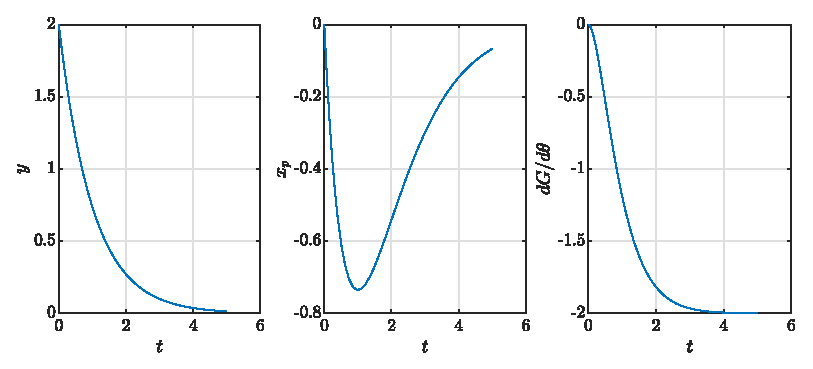
\includegraphics[width=0.9\textwidth]{Figures/Ugf21b.eps}
	
	The code implementation in Matlab is as follows:
	\begin{lstlisting}
		y0 = [2, 0, 0]; theta = 1;
		
		f = @(t,y) [-theta*y(1); ... y
		-theta*y(2) - y(1);... Xp
		2*y(1)*y(2)... dG/dp
		]; 
		
		options = odeset('RelTol',RelTol,'AbsTol',AbsTol); % setting finer tolerences
		[t,yval] = ode45(@(t,y) f(t,y),[0 5],y0);
	\end{lstlisting}
	\item[(c)] Adjoint sensitivity analysis
	
	The implementation of the Adjoint sensitivity analysis in Matlab is presented as follows:
	\begin{align*}
		\text{let, }F &= \dot y + \theta\,y,\ & g&= y^2, \text{ then,}\\
		F_x &= \theta\ \&\ \dot F_x = 1, & g_x &= 2\,y		
	\end{align*}
	Now, we need to solve for $\lambda$ backwards from $T$
	\begin{align*}
		(-\lambda\,\dot F_x)' + \lambda\,F_x + g_x &= 0,
	\end{align*}
	Here we define the following:
	\begin{align*}
		z(\tau) &= x\,(T - \tau),\ t = T - \tau;\ \text{where,}\\
		\dot x &= -y(T -t) = -\dot y(\tau), & x(t) &= y(T-\tau) = y(\tau),\ \text{and,}\\
		-y(\tau) &= -\lambda(T-\tau), & y(\tau) &= \theta\,\lambda(T-\tau),\ \text{and,}\\
		g_x &= 2\,y(t-\tau).
	\end{align*}
	Using $\lambda$, we calculate $\frac{dG}{d\theta}$ using the following relation:
	\begin{align*}
		\frac{dG}{d\theta} &= \int g_p - \lambda(t)\,F_p dt,\text{ where}
		g_p &= -\theta\,y, & F_p &= y
	\end{align*}
	Thus, we get $$\frac{dG}{dt}\Bigg|_{T = 5,\ \theta = 1} = \textbf{-1.9856}$$
	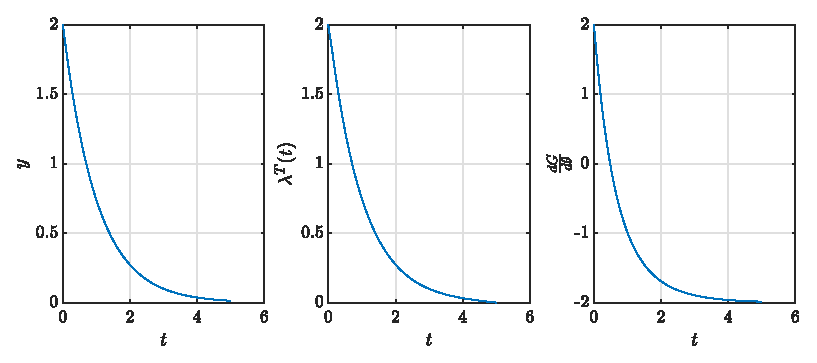
\includegraphics[width=\textwidth]{Figures/Ugf31c.eps}
	The code is presented as follows:
	\begin{lstlisting}
		T = 5; % final time 
		theta = 1; y0 = 2;
		
		f1 = @(t,y) -theta*y; ... y
		
		options = odeset('RelTol',RelTol,'AbsTol',AbsTol); % TOL setting
		[tsim,yval_2] = ode45(@(t,y) f1(t,y),[0 5],y0,options); % solving for y
		
		gx = @(t) interp1(tsim,2*yval_2,t,'spline'); % 2*y(tau) //ERROR should be Tau not t
		f2 = @(tau,lambda) -theta*lambda + gx(T - tau); % DE for lambda
		
		lambda_fin = 0; % initital guess based on lambda*Fx' = 0; since Fx' is 1, lambda = 0.
		[tsim_lambda,lambda_val] = ode45(@(t,y) f2(t,y),[0 5],lambda_fin,options); % solving for lambda
		
		tsim_lambda_t = flipud(T - tsim_lambda);
		lambda_t = flipud(lambda_val)'; % flipping the lambda and making it w.r.t t

		x0 = 1*theta*lambda_t(1);% Fx'(0)*Fx(0)*lambda(0)
		
		f3 = @(t,x) -theta*interp1(tsim,yval_2,t,'linear') - interp1(tsim_lambda_t,lambda_t,t,'spline')*interp1(tsim,yval_2,t,'linear'); % dG/dp
		[tsim_dGdp,dGdp_val] = ode45(@(t,y) f3(t,y),[0 5],x0,options); % just integrating
	\end{lstlisting}
\end{enumerate}
The following table presents $\frac{dG}{dt}|_{T = 5,\ \theta = 1}$ using all the three methods of sensitivity analysis.
\begin{center}
	\begin{tabular}{c|c|c}
		Analytical & Forward & Adjoint \\
		\hline
		-1.9990 & -1.9998 & -1.9856
	\end{tabular}
\end{center}
